\documentclass{../../slides-style}

\slidetitle{Комментарии по домашке}{20.09.2023}

\begin{document}
    
    \begin{frame}[plain]
        \titlepage
    \end{frame}
    
    \begin{frame}
        \frametitle{Процесс компиляции в С}
        \framesubtitle{Почему .sln-файл присылать недостаточно}
        \begin{center}
            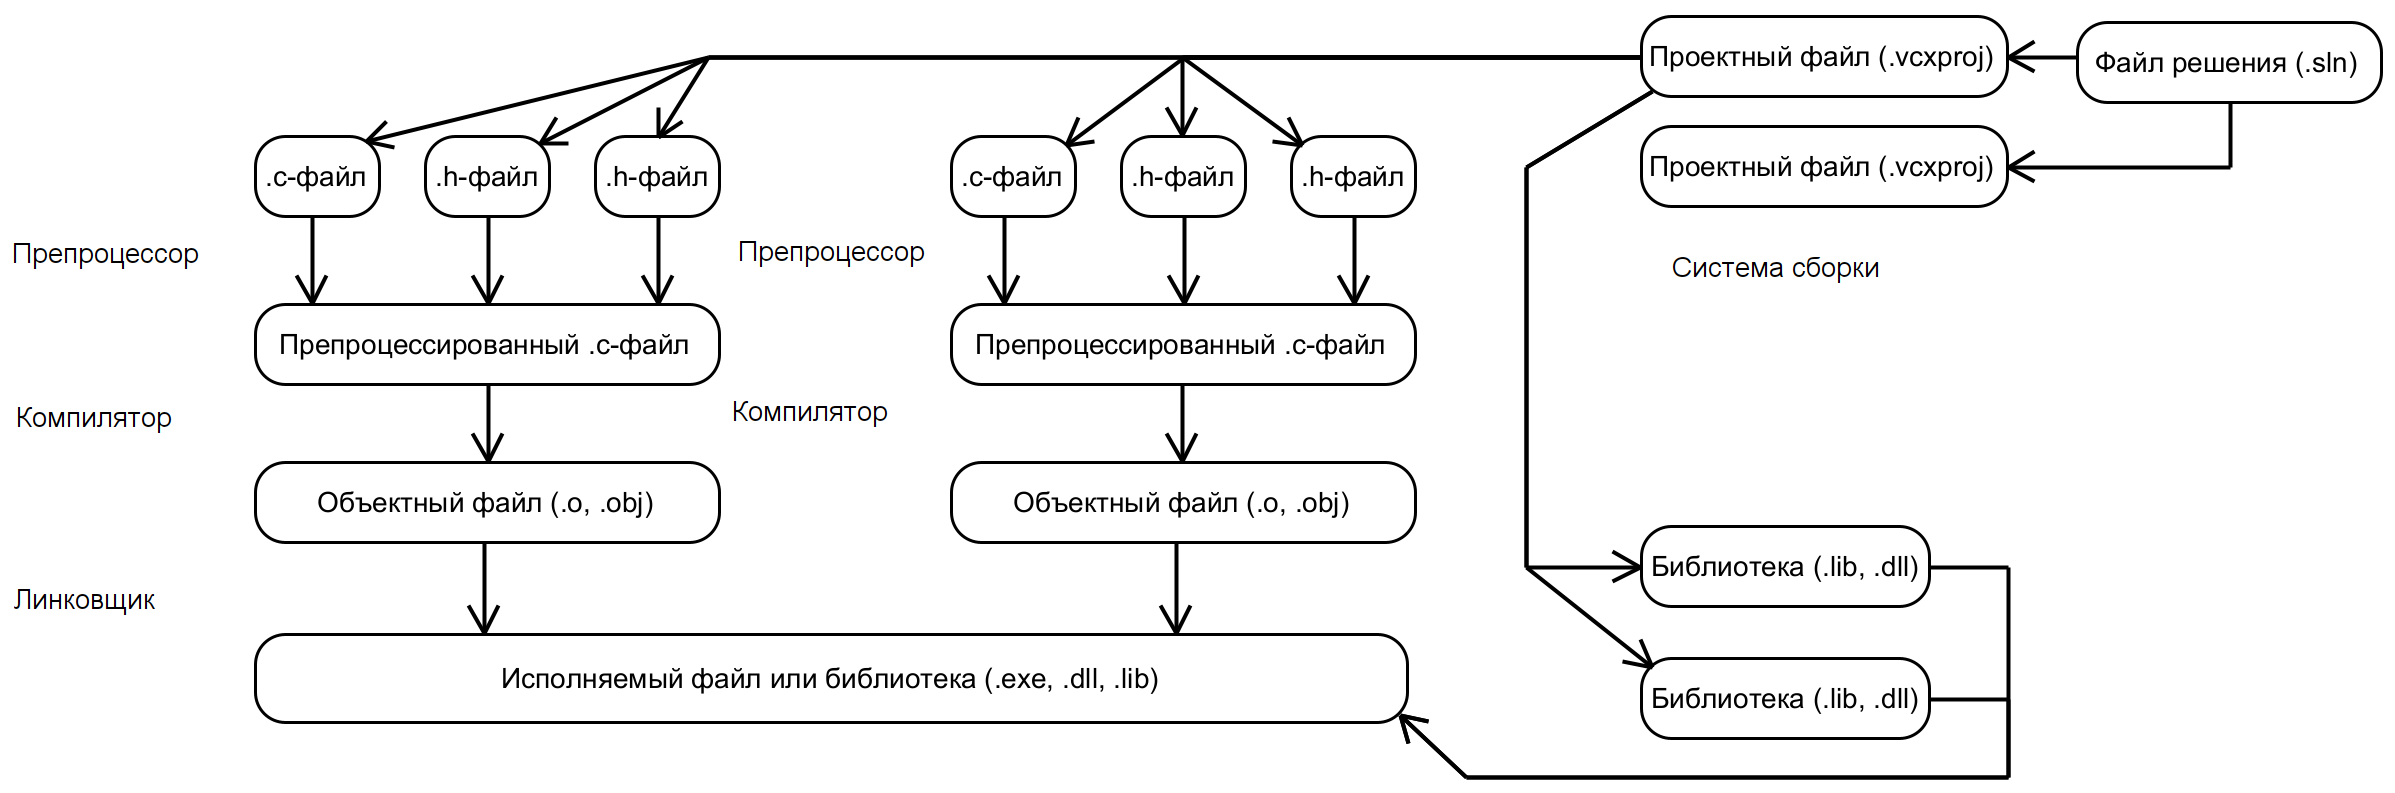
\includegraphics[width=0.95\textwidth]{compilation.png}
        \end{center}
    \end{frame}

    \begin{frame}[fragile]
        \frametitle{Общие замечания}
        \begin{itemize}
            \item Инициализируйте все переменные в месте объявления, всегда
            \item \mintinline{c}|#include| пишется без точки с запятой, это директива препроцессора
            \item 
            \begin{minted}{c}
int n = 0;
scanf("%d", &n);
int array[n];
            \end{minted}
            --- так не работает!
            \item \mintinline{c}|int array[] = {};| тем более не работает
            \item Инициализаторы: \mintinline{c}|int array[10] = {0};| или \mintinline{c}|int array[10] = {1};| или \mintinline{c}|int array[10] = {0, 1, 2, 3, 4, 5, 6, 7, 8, 9};|
            \item Русские буквы: не используйте пока
            \begin{itemize}
                \item Или погуглите про setlocale
            \end{itemize}
        \end{itemize}
    \end{frame}

    \begin{frame}[fragile]
        \frametitle{Ещё рекомендации}
        \begin{itemize}
            \item Тернарный оператор: \mintinline{c}|printf(x == 0 ? "true" :  "false");|
            \item xor: \mintinline{c}|a ^ b ^ b == a|
            \item Инициализация переменных:
                \begin{minted}{c}
int a = 0;
a = (b + c) / 2;
                \end{minted}
            \item \mintinline{c}|printf("%s %d", "Ответ: ", x);| vs \mintinline{c}|printf("Ответ:  %d", x);|
            \item Именованные константы: 
                \begin{minted}{c}
#define SIZE 10
                \end{minted}
            \item Сравнение знаковых и беззнаковых целых: \mintinline{c}{for (int i = 0; i < strlen(s); ++i)}
            \item Булевые переменные --- stdbool.h, bool, true, false
        \end{itemize}
    \end{frame}

    \begin{frame}[fragile]
        \frametitle{И ещё рекомендации}
        \begin{itemize}
            \item Отделяйте логику работы от общения с пользователем --- для переиспользования
            \item \mintinline{c}{int function()} vs \mintinline{c}{int function(void)}
            \item Именование файлов --- тоже в camelCase
            \item Сброс входного потока: \mintinline{c}|scanf("%*[^\n]");| или \mintinline{c}|while (getchar() != '\n') {|
        \end{itemize}
    \end{frame}

    \begin{frame}[fragile]
        \frametitle{if-else и return}
        \begin{minted}{c}
void f(int x) {
    if (x == 0) {
        ...
    } else {
        ...
    }
}
        \end{minted}
        или
        \begin{minted}{c}
void f(int x) {
    if (x == 0) {
        ...
        return;
    } 
    ...
}
        \end{minted}
    \end{frame}

\end{document}

